\subsection{Negativa tal}

Ett negativt tal är bara den additiva inversen av samma tal. Om $a$ är ett reellt tal och $-a$ är dess additiva invers, så är $a+(-a)=0$. Ett sätt att se på det är att den additiva inversen (negativa varianten) av ett tal är lika långt från $0$ på tallinjen, men åt andra hållet. 

Multiplikation får några egenskaper utav detta, som att negativt gånger negativt blir positivt. Att vända dig om och sedan backa blir detsamma som att bara gå rakt fram från början.

Några regler kring detta är då:

\begin{align}
	(-a)(-b) = ab \\
	\frac{(-a)}{(-b)} = \frac{a}{b} \\
	(-a)b = a(-b) \\
	\frac{(-a)}{b} = \frac{a}{(-b)}
\end{align}

\newpage
\subsection{Prioriteringsregler}

Prioriteringsregler har vi, då att om vi fick välja helt fritt så skulle alla få olika svar. Ordningen är såhär:

\begin{enumerate}
	\item Paranteser
	\item Multiplikation/Division 	
	\item Addition/Subtraktion
\end{enumerate}

Om två av samma prioritet är efter varann, börja från vänster.

Ett exempel är 

\begin{align*}
	6\div 2(1+2) = \\
	6\div 2(3) = \\
	6\div 2 \cdot 3 = \\
	3 \cdot 3 = \\
	9
\end{align*}

\newpage
\subsection{Bråk}

Bråk är tal som representeras som kan skrivas som en kvot\footnote{resultatet av en division} av två heltal. Det kan t.ex vara $\frac{3}{7}$, vilket kan tänkas som  \textit{tre sjundedelar}.

\subsubsection{Addition av bråk}
\label{Addition av bråk}
Lättaste metoden för addition av bråk är att skriva om bråken så att de får samma nämnare\footnote{nedre parten hos ett bråk}:

\begin{align}
	\frac{1}{3} + \frac{3}{4} = \\
	\frac{1\cdot 4}{3\cdot 4} + \frac{3\cdot 3}{4\cdot 3} = \label{expre1} \\
	\frac{4}{12} + \frac{9}{12} = \label{expre2} \\
	\frac{13}{12}
\end{align}

Metoden jag brukar använda för att skriva om bråken, är att multiplicera täljaren och nämnaren på det ena bråket, med nämnaren på det andra, och tvärt om. I exemplet ovan så har ena bråket nämnaren 3, så jag multiplicerar täljaren och nämnaren med just 3 på det andra bråket, och tvärt om med talet 4 på det förstnämnda bråket. Genom denna metod får bråken samma nämnare då $ab = ba$, som ses i nämnarna på rad \eqref{expre1} till \eqref{expre2}. Efter det så kan man addera täljarna på bråken.

Addition och subtraktion fungerar likadant här.

\subsubsection{Multiplikation av bråk}

Multiplikation av bråk är mycket enkelt.

\begin{align}
	\frac{a}{b} \cdot \frac{c}{d} = \frac{ac}{bd}
\end{align}

\subsubsection{Division av bråk}
\label{Division av bråk}

Division är en typ av multiplikation, vilket gör denna ganska enkel men aningen klurigare. Division är inversen av multiplikation, så att dividera med $5$ är samma sak som att multiplicera med $\frac{1}{5}$. Detta resulterar i att:

\begin{align}
	\frac{a}{b} \div\frac{c}{d} = \\ 
	\frac{a}{b} \cdot \frac{d}{c} = \\
	\frac{ad}{bc}
\end{align}

Det andra bråket vänder alltså bara på sig vid utbytet av divisionstecken mot multiplikationstecken.

\newpage
\subsection{Potenser}
\label{Potenser}

Potenser kan ses som repeterad multiplikation i vissa fall\footnote{andra definitioner krävs för att inkludera alla reella eller till och med komplexa exponenter. Det kommer först i universitetsmatten.}. Alltså att om exponenten\footnote{En exponent är den övre delen av en potens, alltså det som brukar komma efter man säger \textit{upphöjt till}} $n$ är ett positivt heltal så gäller detta:

\begin{align}
	a^n = a_1 \cdot a_2 \cdot ... \cdot a_n
\end{align}

\textit{Roten ur} kan skrivas på två sätt, där $n$ är ett positivt heltal:

\begin{align}
	\sqrt[n]{a} = a^{\frac{1}{n}}
\end{align}

\newpage
\subsubsection{Potensregler}


Dessa regler gäller för alla tal, alltså inte bara heltal för exponenterna.

\begin{align}
	a^ba^c = a^{b+c} \\
	\frac{a^b}{a^c} = a^{b-c} \\
	(a^b)^c=a^{bc} \\
	(ab)^x=a^xb^x \\
	\left(\frac{a}{b}\right)^x=\frac{a^x}{b^x} \\
	a^{-b} = \frac{1}{a^b} \\
	a^0 = 1
\end{align}

\newpage
\subsection{Ekvationer}

En ekvation är ett typ av påstående, som innehåller en eller fler variabler (okända). Jag kan påstå att $3x+2 = 8$ utan att säga vad $x$ är. Just detta är endast sant om $x=2$.

Ekvationer brukar kräva att man löser ut enskilda variabler i slutändan. Metoden jag brukar ha är att först och efter varje steg se om jag kan förenkla ekvationen genom addition/subtraktion, sedan om det går genom multiplikation/division, och till sist om det går genom potenser.

\paragraph{Exempel 1}

\begin{align*}
	\frac{x}{x+10} = \frac{24}{54}
\end{align*}

Först så letar jag om jag kan göra något med addition/subtraktion, vilket inte hjälper här. Nästa möjlighet är om multiplikation/division kan förenkla något, vilket det kan genom multiplikation av $x+10$ på båda sidor\footnote{Detta förenklar då multiplikation är lättare att hantera än division, så vi vill få bort divisionstecken.}

\begin{align*}
	x = \frac{24}{54}(x+10)
\end{align*}

Nu kollar vi igen. Addition/subtraktion hjälper inget, men multiplikation/division hjälper återigen här. Vi förenklar genom att multiplicera in i parantesen.

\begin{align*}
	x = \frac{24}{54}x + \frac{24}{54} \cdot 10
\end{align*}

Återigen så letar vi. Addition/subtraktion verkar hjälpa denna gång då målet är att få x på samma sida av likhetstecknet. Vi subtraherar med $\frac{24}{54}x$. I samma veva kan vi även multiplicera in $10$ i bråket på höger sida.

\begin{align*}
	x - \frac{24}{54}x = \frac{24}{54} \times 10 \\
	x - \frac{24}{54}x = \frac{240}{54}
\end{align*}

Nu så kikar vi igen. Multiplikation/divison hjälper för att möjliggöra subtraktion av bråken på vänster sida av likhetstecknet, genom att låta dem få samma nämnare som i \ref{Addition av bråk}.

\begin{align*}
	\frac{54}{54}x - \frac{24}{54}x = \frac{240}{54}
\end{align*}

Nu kan vi alltså subtrahera bråken på vänster sida väldigt lätt.

\begin{align*}
	\frac{30}{54}x = \frac{240}{54}
\end{align*}

Här så hjälper inte addition/subtraktion, men multiplikation/division gör. Vi dividerar med $\frac{30}{54}$ för att $x$ ska bli ensam på vänsterledet.

\begin{align*}
	x = \frac{240}{54} \div \frac{30}{54}
\end{align*}

Här så kan vi ändra om från division av bråken till multiplikation av bråken, på sättet beskrivet i \ref{Division av bråk}.

\begin{align*}
	x = \frac{240}{54} \times \frac{54}{30}
\end{align*}

$54$ i nämnaren på första bråket och i täljaren på andra bråket tar ut varann, och resterande steg bör gå rätt smidigt:

\begin{align*}
	x = \frac{240}{30} \\
	x = \frac{24}{3} \\
	x = 8
\end{align*}

\paragraph{Exempel 2}

\begin{align*}
	x^{\frac{1}{3}} = 3
\end{align*}

Här så fungerar inte addition/subtraktion, eller multiplikation/division. Nästa sak att checka är alltså potenser. Här så kan vi använda oss av potensreglerna i \ref{Potenser}, där $(a^b)^c = a^{bc}$, för att ändra exponenten hos $x$ från $\frac{1}{3}$ till $1$.

\begin{align*}
	(x^{\frac{1}{3}})^{3} = (3)^3 \\
	x^{\frac{3}{3}} = 27 \\
	x^1 = 27 \\
	x = 27
\end{align*}

\newpage
\subsection{Pythagoras Sats}
\label{Pythagoras Sats}

Denna är kort, men viktig. 

\begin{theorem}
	För en rätvinklig triangel med sidlängderna $a$ och $b$ för vardera katet\footnote{de kanter som är direkt anslutna med det rätvinkliga hörnet} och $c$ för hypotenusan, så gäller det att 

	\begin{align}
		a^2+b^2=c^2
	\end{align}
\end{theorem}

\newpage
\subsection{Inversfunktion (viktigt till logaritmer)}
\label{Inversfunktion}

En inversfunktion är en funktion som gör exakt motsatt av originalfunktionen. Om $g(x)$ är inversfunktionen till $f(x)$, och $f(x)$ mappar\footnote{med mappar så menar jag att om jag sätter in värdet $1$ i funktionen, alltså att $x=1$, så ger funktionen $f(x)$ ut något värde beroende på värdet jag satte in, och om det är $3$ så mappar $f(x)$ $1 \rightarrow 3$.} $a \rightarrow b$, så mappar $g(x)$ $b \rightarrow a$.

På grund av detta så kan man grafiskt se att en inversfunktion speglas runt linjen y=x till originalfunktionen. En annan konsekvens är att $f(g(x))=x$ då $g(x)$ bara mappar tillbaka igen till det ursprungliga värdet.

\subsubsection{Exempel}

Vi väljer att $f(x) = 2x + 2$. Vi låter $g(x)$ vara inversfunktionen av $f(x)$. Då $f(x)$ är en linjär funktion så kommer inversen av $g(x)$ också vara linjär då $g(x)$ är spegelbilden av $f(x)$ runt linjen $y=x$. Därmed kan vi konstatera att
\begin{align*}
	g(x)=kx+m.
\end{align*}
För att ta reda på $k$ och $m$ så kan vi skapa ett ekvationssystem med hjälp av att vi vet att $g(x)$ är inversen av $f(x)$.
\begin{align*}
	f(0) = 2 \Leftrightarrow g(2) = 0 \\
	f(1)=4 \Leftrightarrow g(4)=1
\end{align*}
Jag väljer att använda additionsmetoden från \ref{Additionsmetoden}.
\begin{align*}
	\begin{cases}
		2k+m = 0 \\
		4k+m = 1
	\end{cases}
\end{align*}
Jag multiplicerar rad 1 med $(-1)$
\begin{align*}
	\begin{cases}
		-2k-m = 0 \\
		4k+m = 1
	\end{cases}
\end{align*}
Jag adderar rad 1 till rad 2
\begin{align*}
	\begin{cases}
		-2k-m = 0 \\
		2k = 1
	\end{cases}
\end{align*}
Jag förenklar rad 2 genom att dividera med $2$
\begin{align*}
	\begin{cases}
		-2k-m = 0 \\
		k = \frac{1}{2}
	\end{cases}
\end{align*}
Jag adderar rad 2, två gånger, till rad 1.
\begin{align*}
	\begin{cases}
		-m = 1 \\
		k = \frac{1}{2}
	\end{cases}
\end{align*}
Jag dividerar rad 1 med $(-1)$
\begin{align*}
	\begin{cases}
		m = -1 \\
		k = \frac{1}{2}
	\end{cases}
\end{align*}
Detta betyder då att
\begin{align*}
	g(x) = \frac{1}{2}x-1.
\end{align*}

Om vi nu tittar på $f(x)$ och $g(x)$ grafiskt så ser det ut såhär:

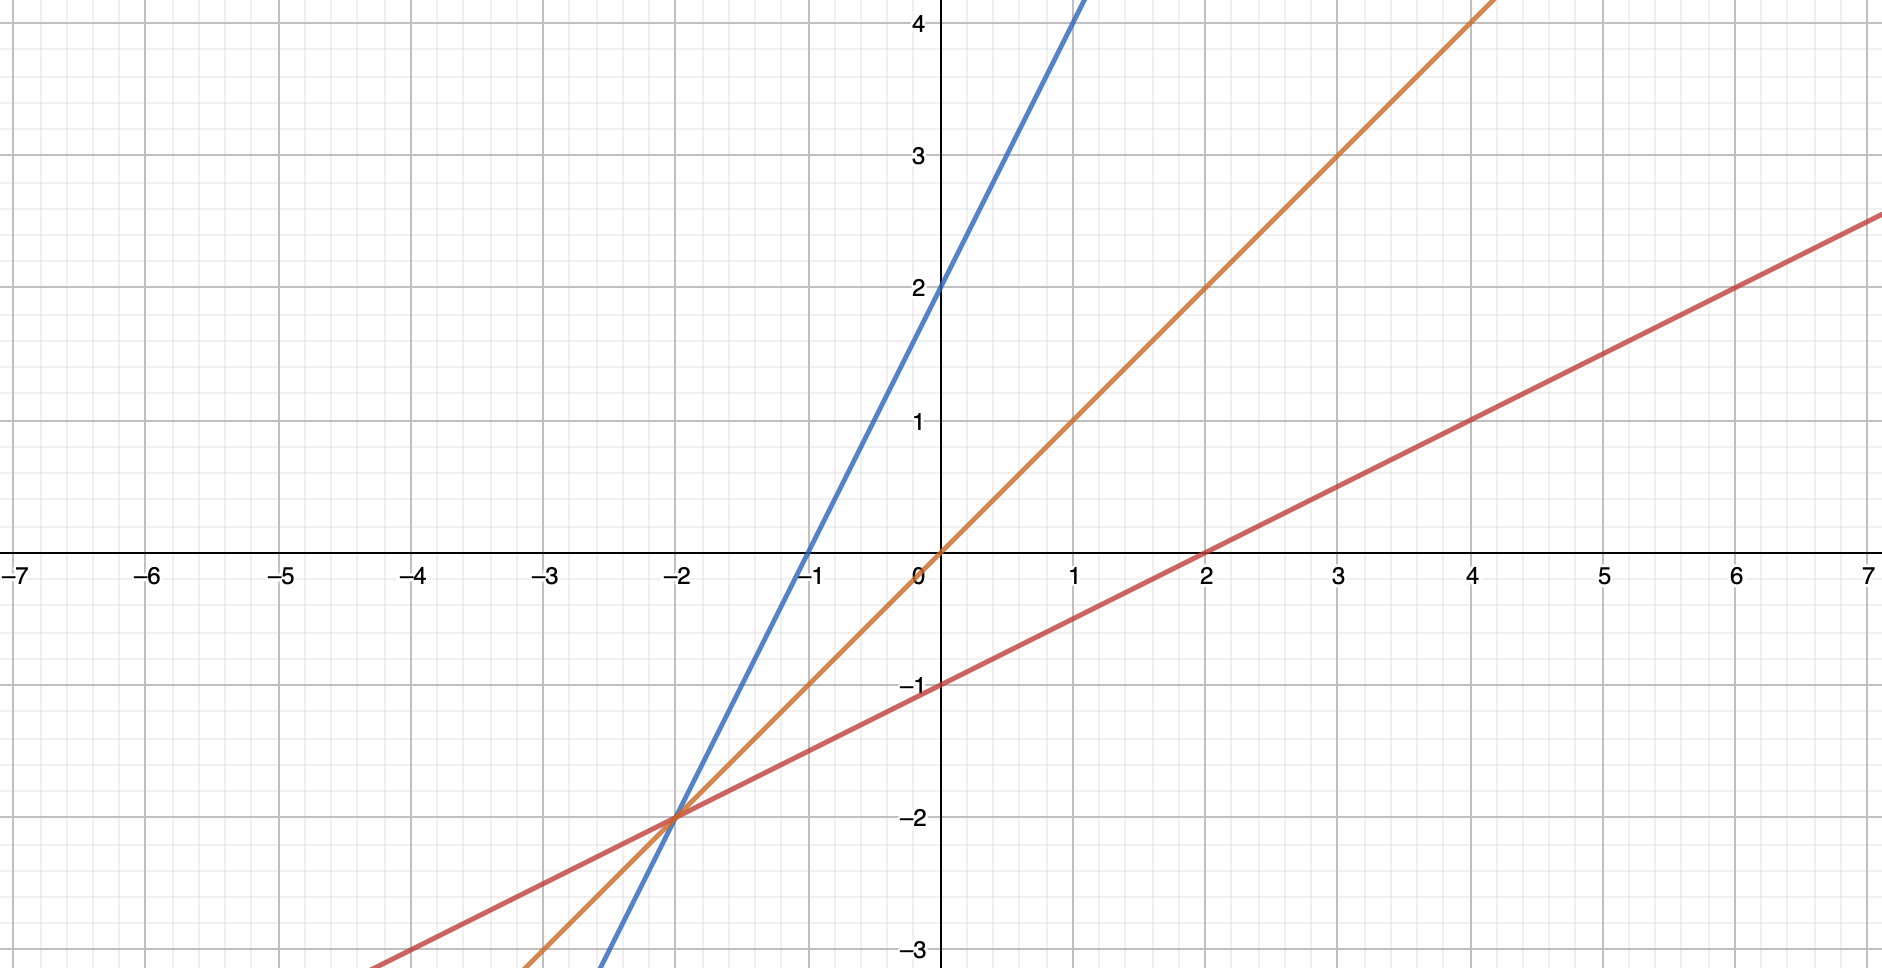
\includegraphics[width=\textwidth]{img/5.png}

I bilden är $f(x)$ den blåa linjen och $g(x)$ är den röda. Linjen som de speglas runt är $y=x$ som är orange här.

Vi kan se i bilden att t.ex så är $f(1)=4$ och att om vi då stoppar in det värde $f(x)$ kastade ut, in i $g(x)$, så får vi $g(4)=1$ vilket gör att vi bara får tillbaka det värde vi hade innan. $g(x)$ är inversen av $f(x)$.






















































